%-----------------------------------------
% Note: Use pdflatex to process this file.
%-----------------------------------------

%\documentclass{article}
\documentclass{hitec}
\usepackage{color,soul}

\usepackage{setspace}
\usepackage{graphicx}
\usepackage{moreverb}    % Defines {listing} environment.
\usepackage{amsmath, amsthm, amssymb, amsbsy, mathtools}
\usepackage{relsize}     % Make letters smaller/larger
\usepackage{alltt}
\usepackage{rotating}
\usepackage{subcaption}
\usepackage{xspace}
\usepackage[section]{placeins}   % For preventing floats from floating to end of chapter.
\usepackage{longtable}   % For splitting long vertical tables into pieces
\usepackage{index}
\usepackage{multirow}
\usepackage{booktabs}    % For table layouts
\usepackage{yhmath}      % For widehat
\usepackage{xcolor}      % Needed for listings package.
\usepackage{listings}
\usepackage[T1]{fontenc}   % so _, <, and > print correctly in text.
\usepackage[strings]{underscore}    % to use "_" in text
\usepackage[pdftex,colorlinks=true,bookmarksnumbered=true]{hyperref}   % Must be last package!

\definecolor{light-gray}{gray}{0.95}
\lstset{backgroundcolor=\color{light-gray}}
\lstset{xleftmargin=0cm}
\lstset{framexleftmargin=0.3em}
\lstset{mathescape=true}
%\lstset{basicstyle = \ttfamily\fontsize{11}{11}\selectfont} 
\lstset{basicstyle = \small}
\lstnewenvironment{code}{}{}

%---------------------------------------------------------------------------------

\definecolor{lightestgray}{gray}{0.99}
\sethlcolor{lightestgray}
\soulregister{\texttt}{1}
\newcommand\dottcmd[1]{\hl{\em#1}\endgroup}
%\newcommand\dottcmd[1]{{#1}\endgroup}
\newcommand{\vn}{\begingroup\catcode`\_=11 \catcode`\%=11 \dottcmd}
\newcommand{\ltt}{\vn{long_term_tracking}\xspace}
\newcommand{\Newline}{\hfil \\}
\newcommand{\sref}[1]{$\S$\ref{#1}}
\newcommand{\Sref}[1]{Sec.~\sref{#1}}
\newcommand{\Th}{$^{th}$\xspace}
\newcommand{\norm}{\text{norm}}
\newcommand{\unnorm}{\text{unnorm}}
\newcommand{\Eq}[1]{Eq.~\ref{#1}}
\newcommand{\tJ}{\widetilde J}
\newcommand{\eps}{{\mathlarger\varepsilon}}
\newcommand{\core}{\text{core}}
\newcommand{\Bf}[1]{{\bf #1}}
\newcommand{\bfN}{\Bf N}

%---------------------------------------------------------------------------------

\renewcommand{\textfraction}{0.1}
\renewcommand{\topfraction}{1.0}
\renewcommand{\bottomfraction}{1.0}

\settextfraction{0.9}  % Width of text
\setlength{\parindent}{0pt}
\setlength{\parskip}{1ex}
%\setlength{\textwidth}{6in}
\newcommand{\Section}[1]{\section{#1}\vspace*{-1ex}}
\newenvironment{display}
  {\vspace*{-1.5ex} \begin{alltt}}
  {\end{alltt} \vspace*{-1.0ex}}

%%% Table of Contents spacing.
\makeatletter
\renewcommand{\l@section}{\@dottedtocline{1}{1.5em}{3.3em}}
\renewcommand{\l@subsection}{\@dottedtocline{2}{3.8em}{4.2em}}
\renewcommand{\l@figure}{\@dottedtocline{1}{1.5em}{3.3em}}
\renewcommand{\l@table}{\@dottedtocline{1}{1.5em}{3.3em}}
\makeatother

%---------------------------------------------------------------------------------

\title{Long Term Tracking Program}
\author{}
\date{David Sagan \\ October 30, 2023}

\begin{document}
\pdfbookmark[1]{Contents}{contents}

\maketitle

\tableofcontents

%---------------------------------------------------------------------------------

\Section{Introduction} 
\label{s:intro}

The \ltt program is for long term (over many turns) tracking of a particle or a beam in a ring. The
\ltt program can track spin as well as simulate such things as element misalignments, wake fields,
higher order mode cavity resonances, energy ramping, beta squeezing, etc. The output of the program
will be such things as turn-by-turn particle tracks or beam statistics including beam sizes and
polarizations.

The \ltt program is built atop the Bmad software toolkit \cite{b:bmad}. The Bmad toolkit is a
library, developed at Cornell, for the modeling relativistic charged particles in storage rings and
Linacs, as well as modeling photons in x-ray beam lines.

%------------------------------------------------------------------
\Section{Running the Long Term Tracking Program} 
\label{s:run}

The \ltt program comes with the ``Bmad Distribution'' which is a package which contains the Bmad
toolkit library along with a number of Bmad based programs. See the Bmad web site for more details.

See the documentation for setting up the Bmad environment variables at
\begin{code}
  https://wiki.classe.cornell.edu/ACC/ACL/RunningPrograms
\end{code}

The \ltt program comes in two versions: 
\begin{code}
long_term_tracking      ! Single threaded version
long_term_tracking_mpi  ! Multi-threaded version
\end{code}
The first is a single threaded version and the second is a multi-threaded version using MPI.\footnote
  {
Note to Distribution maintainers: The single threaded version will be built when compiling a Bmad
Distribution. If MPI is not enabled (which is the default setting), the MPI version will not be
built.  The MPI version can be built by setting \vn{export ACC_ENABLE_MPI=Y} and then using the
``\vn{mk}'' command in the \vn{bsim} directory to build the executable. See the documentation on the
Bmad web site for more details.
  }

Once the Bmad environment variables have been set, the syntax for invoking the single threaded
version of the \ltt program is:
\begin{code}
long_term_tracking {<master_input_file_name>}
\end{code}
Example:
\begin{code}
long_term_tracking my_input_file.init
\end{code}
The \vn{<master_input_file_name>} optional argument is used to set the master input file name. The
default value is ``\vn{long_term_tracking.init}''. The syntax of the master input file is explained
in \sref{s:input}.

Example input files are in the directory (relative to the root of a Distribution):
\begin{code}
bsim/long_term_tracking/example
\end{code}

When running the MPI version threaded over multiple computers, the details of how to start the process will
vary depending upon the installation. See your local Guru for details. When running on a single machine, 
the typical command will look like
\begin{code}
mpiexec -n <num_processes> long_term_tracking_mpi {<master_input_file_name>}
\end{code}
where \vn{<num_processes>} is the number of processes. 

%------------------------------------------------------------------
\Section{Definition of Some Terms}
\label{s:def}

\begin{description}
\item[Beam] \Newline
A \vn{beam} consists of a train \vn{bunches}. Each \vn{bunch} consists of a number of particles contained
within one RF bucket.
%
\item[Radiation Damping and fluctuations] \Newline
At a given particle position, the energy kick $dE$ that a particle receives due to emission of
radiation can be decomposed into two parts. One part is the average kick $dE_d$ and the other part
is a random fluctuation $dE_r$ around the average 
\begin{equation}
  dE = dE_d + dE_r
\end{equation}
An analysis shows that the average part $dE_d$ leads to damping with respect to the closed orbit and
the fluctuation part leads to excitation of the particle motion. Over many turns, there is an
equilibrium reached which gives a particle beam its natural size. While it is not physically
possible to have radiation damping without excitation and vice versa, this can be done with ease in
a simulation.
%
\item[PTC] \Newline
PTC is a library developed by \'Etienne Forest to handle Taylor maps to any arbitrary order. In
particular, PTC is used for constructing maps for the \vn{long_term_tracking} program. PTC can also
be used to do element-by-element tracking.
\end{description}

%------------------------------------------------------------------
\Section{Simulation Modes}
\label{s:sim.modes}

There are a number of simulation ``modes'' which determine what is done by the program. The
simulation mode is set by the \vn{ltt%simulation_mode} parameter in the master input file
(\sref{s:input}).  Possible settings of \vn{ltt%simulation_mode} are:
\begin{code}
"CHECK"       ! Quick tracking check.
"SINGLE"      ! Tracking a single particle.
"INDIVIDUAL"  ! Tracking a set of particles one at a time.
"BEAM"        ! Beam (multi-particle) tracking.
"STAT"        ! Lattice statistics (no tracking done).
\end{code}

\begin{description}
\item["CHECK"] \Newline
In this mode, a particle is tracked from \vn{ltt%ele_start} to \vn{ltt%ele_stop} three times using a
different tracking method each time. The three tracking methods are 1) using a set of maps
(\sref{s:map}), and element-by-element tracking using 2) \vn{Bmad} and 3) \vn{PTC}. The results are
then printed to the terminal. This mode can be used to get a sense of how the three different
methods compare to each other. 

The starting coordinates are set by \vn{beam_init%center} and \vn{beam_init%spin} unless
\vn{beam_init%use_particle_start} is set to True (the default is False). In this case, the
\vn{particle_start} commands in the lattice file are used to set the starting position. In both
cases, if \vn{ltt%add_closed_orbit_to_init_position} is set to True, the closed orbit will be added
in to the initial position.

Included in the output is the transfer matrix
(Jacobian) with respect to the tracked orbit for each of the three tracking methods. These transfer
matrices are computed using finite differences when the starting position is varied. The variation
used in the computation can be specified by setting in the master input file the vector
\vn{bmad_com%d_orb}. This vector has 6 components, one for each phase space component. That is,
\vn{bmad_com%d_orb(1)} sets the variation of the $x$ phase space component, etc.

No data files are produced in this mode.

Radiation fluctuations are turned off in this mode but radiation damping will still be applied if
turned on.

%
\item["SINGLE"] \Newline
In this mode a single particle is tracked for \vn{ltt%n_turns} turns. The starting coordinates are
determined in the same way as is done with the \vn{"CHECK"} mode.

The name of the data file is set by the \vn{ltt%phase_space_output_file} parameter
(\sref{s:input}). The particle position will be output every \vn{ltt%particle_output_every_n_turns}
turns. If this parameter is zero or negative, the position will be outputted at every element.
%
\item["INDIVIDUAL"] \Newline
A set of particles are tracked one-by-one until lost (or until the maximum number of turns set by
the user is reached). Unlike \vn{"BEAM"} mode, no statistics are recorded. Rather the output is the
final position of the particles. The \vn{"INDIVIDUAL"} mode is useful for the situation when there
is ramping (\sref{s:ramp}) and individual are seeing different guide fields due to the time
separation between particles. Specifically, the \vn{"INDIVIDUAL"} mode is useful for simulating
resonant slow extraction.
%
\item["BEAM"] \Newline
In this mode a particle beam is tracked for \vn{ltt%n_turns} turns. Beam statistics are recorded
periodically as set by the user.
%
\item["STAT"] \Newline
In this mode statistics about the lattice are calculated. No long term tracking is done.

Three data files are produced: 
\begin{code}
twiss.dat         ! Twiss parameters
coupling.dat      ! Coupling parameters
closed_orbit.dat  ! Closed orbit
\end{code}
\end{description}

%------------------------------------------------------------------
\Section{Tracking Methods}
\label{s:track.methods}

When tracking with \vn{ltt%simulation_mode} set to \vn{"SINGLE"} or \vn{"BEAM"}, the setting of the
parameter \vn{ltt%tracking_method} determines how particles are tracked. Possible settings are:
\begin{code}
"MAP"     ! Tracking using maps.
"PTC"     ! Element-by-element tracking with PTC. Slow.
"BMAD"    ! Element-by-element tracking using Bmad. Default. Slow.
\end{code}

which is used to determine if tracking is done using a map or not. If a map is used, the order of
the map (the degree at which the Taylor series comprising the map are truncated) is given by
\vn{ltt%map_order} parameter. A larger map order will mean better accuracy at the expense of more
computation time. Tracking using a map will be extremely quick compared to element-by-element
tracking. However, map tracking can be inaccurate if the map order is too small or the particle
amplitude is too large.

Only the \vn{BMAD} method is able to handle a machine that is being ramped (\sref{s:ramp}). That is,
when \vn{ltt%ramping_on} set to True. The program will detect if there is a conflict and issue an
error message and stop.

%------------------------------------------------------------------
\Section{Map Tracking}
\label{s:map}

The \ltt program uses the PTC/FPP library of \'Etienne Forest to handle Taylor maps which can be
constructed to any arbitrary order. Maps will transport both orbital and spin coordinates.  In
particular, PTC is used for constructing the map(s) used for tracking when the
\vn{ltt%tracking_method} parameter is set to "\vn{MAP}" (\sref{s:sim.params}). PTC tracking is also
used when \vn{ltt%tracking_method} is set to "\vn{PTC}". In this case, tracking is done
element-by-element using symplectic integration.

Note: Using maps is not compatible when a machine is being ramped (\sref{s:ramp}).

Sometimes it is convenient to exclude certain lattice elements from a map. For example, the
beam-beam interaction is highly non-linear so excluding any \vn{beambeam} elements can improve map
accuracy at larger amplitudes. Which elements are excluded is determined by the setting of
\vn{ltt%exclude_from_maps} which is a list of what elements are to be excluded. Elements can be
excluded for a number of reasons. When an element is excluded, multiple maps are created, one for
each of the sections of the lattice where there are no excluded elements. In this case, tracking
consists of using a map to track from one excluded element to the next followed by tracking through
the excluded element.

{\em Important!} Maps cannot model RF elements that have a frequency not commensurate with the
one-turn frequency. The reason for this is that a map is just a function that maps the particle's
starting phase space coordinates to the particle's ending coordinates independent of how many turns
the particle has been tracked. But if an RF element has a frequency not commensurate with the
one-turn frequency the kick given a particle going through the element will depend upon the turn
index. Maps can be used to model a lattice with such RF elements, but in this case such elements
must be excluded from be incorporated in any map by setting \vn{ltt%exclude_from_maps} appropriately.

Depending upon how things are setup, a \vn{PTC} map can include radiation damping and fluctuations
effects. \footnote
  {
Radiation fluctuations are included by actually using two maps to track a particle from one point to
the next. One map represents the transport with damping and the second map represents the
fluctuations. When a particle is tracked, the first map with damping is applied and then the second
map is applied using six random numbers.
  }
Damping and excitation are controlled by two parameters that can be set in the master input file:
\begin{code}
bmad_com%radiation_damping_on
bmad_com%radiation_fluctuations_on
\end{code}

The problem with trying to use a map to track a particle's spin when there are radiation effects
present is that a map may not properly model the effect of the radiation fluctuations on the spin
precession (radiation damping is not problematic in itself but that is small comfort). To get around
this, the switch \vn{ltt%split_bends_for_stochastic_rad} may be set True. In this case, all bend
elements are split in the center and special radiation marker elements are placed in between the
split bends. These radiation marker elements are excluded when constructing maps so the result is
many maps whose boundaries will be at the bend centers. When tracking, the maps will not incorporate
stochastic radiation effects (but will still have radiation damping) and a stochastic radiation
kick will be put in at the radiation marker elements as well as any other elements that are excluded
from the maps.

This technique of bend splitting for the purposes of including radiation effects was originally
implemented in a program called \vn{SLICK} and later in the offshoot program \vn{SLICKTRACK}. As
such, this algorithm is known as \vn{SLICK} tracking. A drawback with \vn{SLICK} tracking is the
number of maps needed to track a particle over one turn may be considerably more than just using one
map (essentially there will be one map for every bend in the lattice). This will lengthen
computation times. This being so, it is recommended that \vn{SLICK} tracking only be used when
needed. That is, when both radiation effects and spin tracking are to be simulated. \vn{SLICK}
tracking is also potentially problematical in that radiation effects are not taken into account for
non-dipole elements that are included in any map. If there are any such elements (for example,
wiggler elements), these elements should be excluded from being included in any map.

Maps are saved to a file for use if the program is rerun. For linear maps, an ASCII file
can be produced by setting \vn{ltt%map_ascii_output_file}.

%------------------------------------------------------------------
\Section{Tuning Map and PTC Tracking Parameters}
\label{s:map.tuning}

When tracking using maps or element-by-element with PTC there are a few points to keep in
mind. First is that \vn{PTC} tracks through a lattice element step by step. This is true for both
map creation and symplectic integration. This means that the setting of the element parameter
\vn{integrator_order}\footnote
  {
Note: Valid settings for \vn{integrator_order} are 2, 4, and 6
  }
or \vn{num_steps} (or \vn{ds_step}) for each element will affect the accuracy and speed of the
computations. Bmad tries to choose reasonable default settings for the integrator order and number
of steps however the calculation is not perfect. To make sure that the integrator order and number
of steps is set properly, vary both and choose values (which can be different for different
elements) such that the number of steps and integrator order is minimal (to minimize computation
time) while at the same time is large enough so that results do not change significantly if the
number of steps or is varied. Generally it is much better to use a large integrator order and a
small step size rather than vice versa with the proviso that for elements with a longitudinally
varying field (think wigglers or undulators), the step size must be small compared to the typical
longitudinal length scale over which the field is varying (this length scale is the pole period
length with with wigglers and undulators).

Another thing to keep in mind is that whether a map will give accurate results is dependent on a
number of factors. One factor is the order of the map. Generally higher order is better but will
take more computation time. When the lattice is tracked using a single map, the tracking is only
valid when the tracked particles are far from any strong resonances. That is, if you are interested
in tracking halo particles, you probably should not be using a single map.

In terms of speed, using maps will be the fastest, using standard Bmad tracking will be much
slower, and using PTC element-by-element tracking will be slowest.

In terms of symplecticity, both the PTC tracking and map tracking will be symplectic.
Bmad is not symplectic but the deviation from symplecticity is generally fairly small. If the
radiation effects are large enough, the radiative stochastic noise will negate any non-symplectic
effects and standard Bmad tracking can be used. A very rough rule of thumb is that if the damping times
or the number of turns tracked are under 100,000 turns then Bmad standard tracking can be used.

PTC element-by-element tracking cannot be done when using the MPI version of the \ltt program.

%------------------------------------------------------------------
\Section{Correcting the Orbit when Radiation is Present}

In storage rings, When radiation damping is simulated, the orbit that is flat when there is no
radiation will show a ``sawtooth" pattern'' in a plot of beam energy versus position. This will lead
to a nonzero orbit. In an actual ring, the non-zero orbit will be compensated using steerings. Thus,
to simulate the actual ring, compensating steerings should be added to the simulated lattice as
well. How to do this is covered in the Bmad and Tao Cookbook available from the Bmad web site.

%------------------------------------------------------------------
\Section{Time Ramping --- Time Varying Element Parameters}
\label{s:ramp}

``\vn{Ramping}'' is the situation where lattice parameters are changing as a function of time over
many turns. Ramping examples include changing magnet and RF strengths to ramp the beam energy or
changing magnet strengths to squeeze beta at the interaction ponit of a colliding beam
machine. Additionally, random variations of machine parameters with time can be implemented with
ramper elements to simulate such things as ground motion and RF phase noise.

Ramping is accomplished by defining \vn{ramper} elements in the lattice file and using \vn{time} as
a variable. When tracking through an element, the particle time will be used to set all \vn{time}
ramper variables. Example:
\begin{code}
ramp_e: ramper = \{*[e_tot]:\{4e+08, 4.00532e+08, 4.01982e+08, ...\}\},
              var = \{time\}, x_knot = \{0, 0.001, 0.002, ...\}

amp = 1e9;  omega = 0.167;  t0 = 0.053
ramp_rf: ramper = \{rfcavity::*[voltage]:amp*sin(omega *(time + t0)),
      rfcavity::*[phi0]:0.00158*time^2 + 2*q \}, var = \{time, q\}
\end{code}
The ``\vn{*[e_tot]}'' construct in the definition of \vn{ramp_e} means that the ramper will be
applied all elements (since the wild card character ``\vn{*}'' will match to any element name), and
it is the element's \vn{e_tot} attribute (the element's reference energy) that will be varied.
In the above example, the \vn{ramp_rf} ramper will be applied to all \vn{rfcavity} elements with
the cavity voltage and phase (\vn{phi0}) being varied.

To simulate noise, use the \vn{ran()} or \vn{ran_gauss()} functions in a slave expression. Example:
\begin{code}
  quake: ramper = \{*[y_offset]: 1e-5*ran_gauss()\}, var = \{\}
\end{code}
In this case no ramper variable is needed. 
When a bunch passes through an element, the slave expression \vn{1e-5*ran_gauss()} is evaluated just
once. That is, it is assumed that the frequency spectrum of the noise falls below 1/\vn{dt_bunch}
where \vn{dt_bunch} is the bunch passage time through the element.\footnote
  {
Currently as implemented the noise spectrum from bunch passage to the next bunch passage is
uncorrelated (``white noise''). This may not be a good approximation. Implementation of a random
number generator with non-white power spectrum is currently a long-term project. Please contact a
Bmad maintainer if interested.
  }

In the case where the reference energy \vn{e_tot} or reference momentum \vn{p0c} is being varied, the
effect on an element will depend upon the setting of the element's \vn{field_master} parameter. For
example:
\begin{code}
q1: quadrupole, k1 = 0.3
q2: quadrupole, k1 = 0.3, field_master = T
\end{code}
In this example, \vn{q1} will have its \vn{field_master} parameter set to \vn{False} since the
quadrupole strength was specified using the normalized strength \vn{k1}. With \vn{q1}, since
\vn{field_master} is False, varying the reference energy or momentum will result in the normalized
strength \vn{k1} remaining fixed and the unnormalized strength \vn{B1_gradient} varying in
proportion to the reference momentum. With \vn{q2}, since \vn{field_master} is True, the
unnormalized strength \vn{B1_gradient} will remain fixed and normalized \vn{k1} will vary
inversely with the reference momentum.

There are two modes that can be selected to determine how ramper elements are applied. If
\vn{ltt%ramp_update_each_particle} is set to True, rampers are applied to a given lattice element as
each particle of the beam passes through the element using the time the particle would pass through
the center of the element. This is appropriate if ramping is fast on the time scale of a bunch
passage or if in \vn{"INDIVIDUAL"} or \vn{"SINGLE"} mode. If set to False, rampers are applied to a
given element only once per beam passage using the time of the center of the bunch passing the
center of the element. This is appropriate for parameters that vary slowly on the time scale of a
bunch passage. For example if ramping magnet strengths with energy ramping which occurs over many
turns, calculating once per beam passage should be a good approximation. The default setting of
\vn{ltt%ramp_update_each_particle} is False for \vn{"BEAM"} mode and True for all other modes.

Before a simulation, individual ramper elements may be toggled on or off by setting the element's
\vn{is_on} attribute in the lattice file: 
\begin{code}
ramp_rf: ramper = ...  ! Ramper element defined.
ramp_rf[is_on] = F     ! Ramper element turned off.
\end{code}

If \vn{ltt%ramping_on} is set to True, ramping will be done if \vn{ltt%simulation_mode} is set to
"\vn{BEAM}" or "\vn{SINGLE}". Ramping will be ignored in the other modes.

\ltt program parameters that affect ramping in the simulation are:
\begin{code}
ltt%ramping_on
ltt%ramping_start_time
\end{code}

When ramping, the \vn{ltt%simulation_mode} (\sref{s:track.methods}) must be set to "\vn{BMAD}". The
program will detect if there is a conflict and issue an error message and stop.


The \vn{ltt%ix_turn_start} parameter can be used to start tracking at any turn. This can be useful if a
simulation is accidentally interrupted. In this case the beam positions can be saved by setting
\begin{code}
  ltt%beam_binary_output_file
  ltt%beam_output_every_n_turns
\end{code}

%------------------------------------------------------------------
\Section{Initial Particle Positions}
\label{s:init.pos}

When the \vn{ltt%simulation_mode} (\sref{s:sim.modes}) is set to \vn{"SINGLE"} or \vn{"CHECK"}, the
initial particle position will be set to the initial beam center position. The parameters that are used to
determine the beam center position are
\begin{code}
beam_init%center           ! (x, px, y, py, z, pz)
beam_init%spin             ! (Sx, Sy, Sz)
beam_init%use_particle_start 
ltt%add_closed_orbit_to_init_position
\end{code}
If \vn{beam_init%use_particle_start} is set to \vn{True}, instead of using the parameters
\vn{beam_init%center} and \vn{beam_init%spin}, the \vn{particle_start} parameters that are set in
the lattice file will be used.

If the \vn{ltt%add_closed_orbit_to_init_position} logical is set to \vn{True}, the closed
orbit position is added in to the center position calculation.

When the \vn{ltt%simulation_mode} is set to \vn{"BEAM"}, the initial particle positions are calculated
using the \vn{beam_init} structure as discussed in the \vn{Beam Initialization} chapter of the Bmad
manual. Like the other modes, if the \vn{ltt%add_closed_orbit_to_init_position} logical is set to
\vn{True}, the closed orbit position is added to the initial particle positions. To read in a file
with beam particle positions, set the \vn{beam_init} structure appropriately. Example:
\begin{code}
beam_init%file_name = 'beam_particle_file.init'
\end{code}

In all cases, tracking will start at the lattice element set by \vn{ltt%ele_start}.

The \vn{beam_init} structure:
\begin{code}
type beam_init_struct
  character(200) :: position_file = ''       ! Initialization file name.
  character distribution_type(3)             ! "ELLIPSE", "KV", "GRID", "".
  type (ellipse_beam_init_struct) ellipse(3) ! For ellipse beam distribution
  type (kv_beam_init_struct) KV              ! For KV beam distribution
  type (grid_beam_init_struct) grid(3)       ! For grid beam distribution
  logical use_particle_start = F     ! Use particle_start?
  character random_engine            ! "pseudo" (default) or "quasi". 
  character random_gauss_converter   ! "exact" (default) or "quick". 
  real center(6) = 0                 ! Bench center offset.
  real center_jitter(6) = 0          ! Bunch center rms jitter
  real emit_jitter(2)   = 0          ! %RMS a and b-mode emittance jitter
  real sig_z_jitter     = 0          ! bunch length RMS jitter 
  real sig_pz_jitter     = 0         ! pz energy spread RMS jitter 
  real random_sigma_cutoff = -1      ! -1 => no cutoff used.
  integer n_particle = 0             ! Num of simulated particles per bunch.
  logical renorm_center = T          ! Renormalize centroid?
  logical renorm_sigma = T           ! Renormalize sigma?
  real(rp) spin(3) = 0, 0, 0         ! Spin (x, y, z)
  real a_norm_emit = 0               ! a-mode normalized emittance
  real b_norm_emit = 0               ! b-mode normalized emittance
  real a_emit = 0                    ! a-mode emittance
  real b_emit = 0                    ! b-mode emittance
  real dpz_dz = 0                    ! pz vs z correlation.
  real dt_bunch = 0                  ! Time between bunches.
  real sig_z = 0                     ! Z sigma in m.
  real sig_pz = 0                    ! pz sigma.
  real bunch_charge = 0              ! Charge in a bunch.
  integer n_bunch = 0                ! Number of bunches.
  character species = ""             ! Species to track.
  logical full_6D_coupling_calc = F  ! Use 6x6 1-turn mat to match 
                                     !              the distribution?  
  logical use_t_coords = F  ! If true, the distributions will be 
                            !   calculated using time coordinates
  logical use_z_as_t   = F  ! Only used if use_t_coords = T:
                            !   True:  The z coordinate stores the time.
                            !   False: The z coordinate stores the s-position.
end type
\end{code}

%------------------------------------------------------------------
\Section{Fortran Namelist Input}
\label{s:namelist}

Fortran namelist syntax is used for parameter input in the master input file. The general form of a
namelist is
\begin{code}
&<namelist_name>
  <var1> = ...
  <var2> = ...
  ...
/
\end{code}
The tag \vn{"\&<namelist_name>"} starts the namelist where
\vn{<namelist_name>} is the name of the namelist. The namelist ends
with the slash \vn{"/"} tag. Anything outside of this is
ignored. Within the namelist, anything after an exclamation mark
\vn{"!"} is ignored including the exclamation mark. \vn{<var1>},
\vn{<var2>}, etc. are variable names. Example:
\begin{code}
&place 
  section = 0.0, "arc_std", "elliptical", 0.045, 0.025 
/
\end{code}
here \vn{place} is the namelist name and \vn{section} is a
variable name.  Notice that here \vn{section} is a ``structure'' which
has five components -- a real number, followed by two strings,
followed by two real numbers.

Everything is case insensitive except for quoted strings.

Logical values are specified by \vn{True} or \vn{False} or can be
abbreviated \vn{T} or \vn{F}. Avoid using the dots (periods) that one
needs in Fortran code.

%------------------------------------------------------------------
\Section{Master Input File}
\label{s:input}

The \vn{master input file} holds the parameters needed for running the long term tracking
program. The master input file must contain a single namelist (\sref{s:namelist}) named \vn{params}.
Example:
\begin{code}
&params
  ! Input
  ltt%lat_file   =  "lat.bmad"     ! Bmad lattice file
  ltt%ramping_on = F
  ltt%ramp_update_each_particle = F
  ltt%ramping_start_time = 0

  ! Simulation parameters
  ltt%simulation_mode           = "BEAM"
  ltt%tracking_method           = "BMAD"
  ltt%ele_start                 = ""
  ltt%ele_stop                  = ""      ! Used for "CHECK" simulation_mode 
  ltt%n_turns                   = 1000
  ltt%ix_turn_start             = 0
  ltt%ix_turn_end               = -1
  ltt%map_order                 = 5
  ltt%rfcavity_on               = T
  ltt%timer_print_dtime         = 300
  ltt%random_seed               = 0
  ltt%ptc_aperture              = 0.1, 0.1
  ltt%exclude_from_maps         = "beambeam::*"
  ltt%action_angle_calc_uses_1turn_matrix = F
  ltt%split_bends_for_stochastic_rad = F
  ltt%symplectic_map_tracking   = F
  ltt%set_beambeam_z_crossing   = F
  ltt%use_rf_clock              = F
  ltt%dead_cutoff               = 0.99
  ltt%b_emittance               = 1e-9       ! Used with space charge calc.
  ltt%debug                     = F
  bmad_com%spin_tracking_on     = T       ! See Bmad manual for 
  bmad_com%radiation_damping_on = F   !    bmad_com parameters.
  bmad_com%radiation_fluctuations_on = F 

  ! Beam initialization
  ltt%add_closed_orbit_to_init_position = T
  beam_init%use_particle_start = F
  beam_init%center = 0, 0, 0, 0, 0, 0
  beam_init%n_particle = 10
  beam_init%spin = 0, 0, 0        ! See Bmad manual for complete list
  beam_init%a_emit = 1e-8         !    of beam_init_struct parameters.
  beam_init%b_emit = 1e-8
  beam_init%sig_z = 1e-4
  beam_init%sig_pz = 1e-4

  ! Output parameters
  ltt%phase_space_output_file = ""
  ltt%action_angle_output_file = ""
  ltt%beam_binary_output_file = "beam.dat"
  ltt%averages_output_file = "average.dat"
  ltt%custom_output_file = ""
  ltt%per_particle_output_file = ""
  ltt%averages_output_every_n_turns = 200
  ltt%particle_output_every_n_turns = 200
  ltt%beam_output_every_n_turns = 200
  ltt%only_live_particles_out = T
  ltt%core_emit_cutoff   = 0.2, 0.5
  ltt%core_emit_combined_calc = T
  ltt%print_on_dead_loss = -1
  ltt%map_file_prefix = "ltt"
  ltt%map_ascii_output_file = ""

  ltt%column(1) = "n_turn", "N_turn", "i7"
  ltt%column(2) = "rf0##1[voltage]", "Volt", "f10.0"
  ltt%column(3) = "rf0##1[phi0] + z/rf0##1[rf_wavelength]", "dPhi", "f12.8"
/
\end{code}

The namelist parameters can be divided into three categories: Input files, output parameters, and
simulation parameters.

%----------------------------------------------------
\subsection{Simulation Parameters}
\label{s:sim.params}

Parameters in the master input file that affect the simulation are:
\begin{description}

\item[ltt\%action_angle_calc_uses_1turn_matrix] \Newline
If set \vn{False} (the default), the conversion matrix ($\bfN^{-1}$ matrix) from $(x, p_x, y, p_y,
z, p_z)$ phase space coordinates to action-angle coordinates is calculated from the beam sigma
matrix as described by Wolski\cite{b:wolski}. That is, the conversion to action-angle coordinates is
affected by lattice nonlinearities and $\bfN^{-1}$ will vary from turn-to-turn. If set to \vn{True},
the conversion matrix is calculated from the 1-turn matrix calculated from the lattice independent of
the beam distribution.
%
\item[ltt\%add_closed_orbit_to_init_position] \Newline
If set \vn{True} (the default), initial particle positions are set equal to the input particle positions
plus the closed orbit position. See Section~\sref{s:init.pos}.
%
\item[beam_init\%...] \Newline
This sets the initial beam distribution. See Section~\sref{s:init.pos}. 

If spin tracking is on (\vn{bmad_com%spin_tracking_on} = T), and if all three components of
\vn{beam_init%spin} are zero, the closed orbit spin direction ($n_0$) is used.

Note: the values of \vn{beam_init%a_emit} and \vn{beam_init%b_emit} along with
\vn{beam_init%bunch_charge} are used in the high energy space charge calculation
(\sref{s:space.charge}). If the emittances set to zero (the default) or negative, the emittance as
calculated via radiation integrals will be used.
%
\item[bmad_com\%...] \Newline
The \vn{bmad_com} structure contains various parameters that affect tracking. For example, whether
radiation damping and fluctuations are included in tracking. A full list of \vn{bmad_com} parameters
is detailed in the Bmad reference manual. Note: \vn{bmad_com} parameters can be set in the Bmad
lattice file as well. \vn{Bmad_com} parameter set in the master input file will take precedence over
parameters set in the lattice file.
%
\item[ltt\%dead_cutoff] \Newline
Sets the cutoff for the number of dead particles below which the simulation will stop. For example,
if \vn{ltt%dead_cutoff} is set to 0.01, when 1\% of the beam has been lost, the simulation will stop. The
default value for \vn{ltt%dead_cutoff} is 0.99
%
\item[ltt\%debug] \Newline
This parameter is used for debugging the program. This is not of interest to the general user.
%
\item[ltt\%ele_start] \Newline
Name or element index of the element to start the tracking. Examples:
\begin{code}
ele_start = "Q3##2"   ! 2nd element named Q3 in the lattice.
ele_start = 37        ! 37th element in the lattice.
\end{code}
The default is to start at the beginning of the lattice. Notice that the tracking starts at the
downstream end of the element so the first element tracked through is the element after the chosen
one. Also see \vn{ltt%ele_stop}.
%
\item[ltt\%ele_stop] \Newline
Used when \vn{ltt%simulation_mode} is set to \vn{"CHECK"} only. \vn{ttl%ele_stop} sets the stopping
point for tracking to be the downstream edge of the element. Also see \vn{ltt%ele_start}. Default
if not set or set to a blank string is for \vn{ltt%ele_stop} to be equal to \vn{tll%ele_start}.
%
\item[ltt\%exclude_from_maps] \Newline
List of elements to exclude when constructing maps for \vn{SLICK} tracking. These elements will be
individually tracking. The default value is \vn{"beambeam::*"} which excludes any \vn{beambeam}
element. See the Bmad manual section on ``\vn{Matching to Lattice Element Names}'' for details on
the format for such lists.
%
\item[ltt\%ix_turn_start, ltt\%ix_turn_stop] \Newline
These parameters are used to select the starting (\vn{ltt%ix_turn_start}) and stopping
(\vn{ltt%ix_turn_stop} turn number for \vn{"SINGLE"} and \vn{"BEAM"} simulations. This is only
useful when ramping in done (\sref{s:ramp}). \vn{ltt%ix_turn_start} defaults to zero. When
\vn{ltt%ix_turn_end} is set, \vn{ltt%n_turns} is set to \vn{ltt%ix_turn_end} -
\vn{ltt%ix_turn_start}. If \vn{ltt%n_turns} is set, \vn{ltt%ix_turn_end} is set to
\vn{ltt%ix_turn_start} + \vn{ltt%n_turns}.
%
\item[ltt\%lat_file] \Newline
Name of the Bmad lattice file to use. This name is required.
%
\item[ltt\%map_order] \Newline
Map order. See Section~\sref{s:track.methods}. The default is what is set in the lattice
file and if not set in the lattice file the default is 3. Note: \vn{ltt%map_order} is only used when
generating a map.  When a map is read in from a file, the order of this map is independent of the
current setting of \vn{ltt%map_order}.
%
\item[ltt\%n_turns] \Newline
Number of turns to track. Only used with \vn{"SINGLE"} and \vn{"BEAM"} modes. Also see
\vn{ltt%ix_turn_start} and \vn{ltt%ix_turn_stop}.
%
\item[ltt\%ptc_aperture] \Newline
The PTC code does not have apertures. This being the case, for \vn{ltt%tracking_method} set to
\vn{"MAP"} or \vn{"PTC"}, \vn{ltt%ptc_aperture}, which is a 2-vector, defines \vn{x} and \vn{y}
apertures. The default is 0.1~meter in both the horizontal and vertical. When used, the aperture is
applied at the beginning/end of the lattice. PTC has an internal aperture of 1.0~meter. To be safe,
the \ltt program will additionally impose a 0.9~meters aperture independent of the setting of
\vn{ltt%ptc_aperture}.
%
\item[ltt\%ramp_update_each_particle] \Newline
Default is False which means only apply rampers to a given lattice element once per beam passage
(\sref{s:ramp}).
%
\item[ltt\%ramping_on] \Newline
If set to True, \vn{ramper} control elements will be use to modify the lattice during tracking
(\sref{s:ramp}). Default is False.
%
\item[ltt\%ramping_start_time] \Newline
The starting (offset) time used to set \vn{ramper} elements. This enables simulations to start in the middle
of a ramp cycle. Default is 0.
%
\item[ltt\%random_seed] \Newline
The random number seed used by the random number generator. If set to 0, the
system clock will be used. That is, if set to 0, the output results will vary from run to run.
%
\item[ltt\%rfcavity_on] \Newline
If set to \vn{False}, the voltage on all RF cavity elements will be turned off. Default is \vn{True}.
%
\item[ltt\%set_beambeam_z_crossing] \Newline
If True (default is false), set the \vn{z_crossing} parameter of any \vn{beambeam} element in the
lattice to the phase space $z$ value of the closed orbit? See the Bmad manual for a discussion of
the \vn{z_crossing} parameter. Generally, \vn{ltt%set_beambeam_z_crossing} should be set True.
%
\item[ltt\%simulation_mode] \Newline
Sets the simulation mode for the program. See Section~\sref{s:sim.modes} for more details.
%
\item[ltt\%split_bends_for_stochastic_rad] \Newline
Use a stochastic radiation point in the middle of all the bends instead of including stochastic
radiation effects in the transport maps (\sref{s:map})? Default is False. For testing, can also be
used with non-map tracking.
%
\item[ltt\%symplectic_map_tracking]\Newline
If False (the default), the maps used for tracking will be a set of truncated Taylor series
polynomials. If True, the tracking maps will be derived from the Taylor map by partially inverting
it forming an implicit symplectic map. The advantage of the symplectic map is that it is symplectic.
The disadvantage is that, being an implicit map, the computation time will be longer.
%
\item[ltt\%timer_print_dtime] \Newline
The program will print a tracking status message every so often. The nominal time between status
messages is set by \vn{ltt%timer_print_dtime} which is a number in seconds.
%
\item[ltt\%tracking_method] \Newline
String switch which sets how particles are tracked when the \vn{simulation_mode} is set to
"\vn{BEAM}" or "\vn{SINGLE}". Possible settings are:
\begin{code}
"MAP"     ! Tracking using maps.
"PTC"     ! Element-by-element tracking with PTC. Slow.
"BMAD"    ! Element-by-element tracking using Bmad. Default. Slow.
\end{code}
See sections \sref{s:map} and \sref{s:track.methods} for more details.
%
\item[ltt\%use_rf_clock] \Newline
The \vn{ltt%use_rf_clock} logical is only relavent if Bmad tracking is being used in conjunction with
absolute time tracking and the discussion here assumes Bmad tracking with absolute time tracking.\footnote
  {
See the Bmad manual for a discussion of absolute versus relative time tracking.
  }
If \vn{ltt%use_rf_clock} is set to False (the default), the time used to calculate the phase of any
varying fields is the absolute time which increases turn-by-turn. Over many turns this may lead to
round-off error. For example, with a 10~GHz cavity, if the phase needs to be measured to one part in
$10^5$, it will not be possible to run a simulation past 10~seconds since the double precision
numbers used in the code have an accuracy of $10^{-16}$. 

There are several possible ways to avoid this round-off problem. If all the frequencies of all the time
varying fields are commensurate with the length of the lattice, relative time tracking can be used
which uses the particle's $z$ phase space coordinate as the effective clock.\footnote
  {
Note: Absolute time tracking is not available with PTC. That is, any PTC based tracking is relative
time tracking.
  }
If all frequencies are commensurate with each other, but are not commensurate with the lattice
length, time patches (patch elements that shift the reference time) can be used with relative time
tracking.  Finally, if all the frequencies are commensurate, the ``\vn{RF clock}'' can be used with
absolute time tracking by setting \vn{ltt%use_rf_clock} to True. The RF clock is simply a clock whose
time is reset periodically to be in the range $[0, t_{rf}]$ where $t_{rf}$ is a time period chosen by
Bmad to be commensurate with the frequencies of the time varying fields.\footnote
  {
If not all the frequencies are commensurate, Bmad will make a best choice and the fields that have
frequencies that are not commensurate with the RF clock will use the standard clock instead.
  }
\end{description}

%----------------------------------------------------
\subsection{Output File Parameters}
\label{s:out.files}

Parameters in the master input file that affect the output are:
\begin{description}
%
\item[ltt\%action_angle_output_file] \Newline
The name of the ASCII file (or files) that are created to hold the particle positions in
action-angle coordinates. Used with \vn{ltt%simulation_mode} set to \vn{"BEAM"}. If
\vn{ltt%action_angle_output_file} is blank, no particle output file is created. See
\Sref{s:beam.part.dat} for more details.
%
\item[ltt\%averages_output_file] \Newline
Used with \vn{ltt%simulation_mode} set to \vn{"BEAM"}. 
The \vn{ltt%averages_output_file} parameter sets the prefix used for the file names for the
\vn{averages}, \vn{sigma} and \vn{emittance} data files (\sref{s:beam.ave.dat}).
%
\item[ltt\%averages_output_every_n_turns] \Newline
Sets the number of turns between data rows of data files specified by:
\begin{code}
ltt%averages_output_file  \sref{s:beam.ave.dat}
ltt%custom_output_file    \sref{s:beam.cust.dat}
\end{code}
For particle phase space output, use the \vn{particle_output_every_n_turns} parameter.
%
\item[ltt\%beam_binary_output_file] \Newline
Used with \vn{ltt%simulation_mode} set to \vn{"BEAM"}. This parameter sets the name of the file that
is created to hold particle positions. This is similar to \vn{ltt%phase_space_output_file} but here
the file will be a binary file that is portable to other programs and can also be used as input to
the \ltt program. A beam file will be created every \vn{ltt%beam_output_every_n_turns} turns if this
quantity is positive. Additionally, a beam file will be produced at the end of tracking. A beam file
will be given a suffix \vn{.NNNN.h5} where \vn{NNNN} is the turn number. To save disk space, every
time a new beam file is created, if there is an old beam file it will be deleted. 

To translate to ASCII, use the \vn{beam_file_translate_format} program. Documentation is in any Bmad
Distribution in the file:
\begin{code}
  util_programs/beam_file_translate_format/DOC
\end{code}

To use a beam file that has been generated on a previous run with a new run set \vn{beam_init%file_name}
to the name of the beam file.
%
\item[ltt\%column(:)] \Newline
The \vn{ltt%column(:)} parameters are used to specify the columns of a custom data file
(\sref{s:beam.cust.dat}).
%
\item[ltt\%core_emit_combined_calc] \Newline
Determines how core emittances are calculated. See \Sref{s:core} for more details. The default value
is \vn{True}.
%
\item[ltt\%core_emit_cutoff] \Newline
The \vn{ltt%core_emit_cutoff} parameter is an array of values used to calculate the ``core''
emittances (\sref{s:core}). Up to 40 values can be given. If a value is non-positive, that value and
any value after that are ignored. The default first value is 0.5 and the reset default to
negative. The value of \vn{ltt%core_emit_cutoff} must be
less than or equal to one. Using a value near zero may lead to invalid results if the number of
particle to be retained is too small since there will be statistical fluctuations of order
$1/\sqrt{N_c}$ where $N_c$ is the number of particles in the core. The core emittance will be in the
\vn{.emit} output data file (see \vn{ltt%averages_output_file}).
%
\item[ltt\%custom_output_file] \Newline
A custom output file can be created that records beam and lattice parameters (\sref{s:beam.cust.dat}).
The columns of the file are set by the \vn{ltt%column(:)} parameters.
%
\item[ltt\%map_ascii_output_file] \Newline
For linear maps, An ASCII file of the maps can be produced by setting this parameter.
%
\item[ltt\%map_file_prefix] \Newline
Prefix, including possible directory specification, for creating files in which maps are saved. Map
files are used to quickly retrieve maps previously computed in prior running of the program. The
default prefix is \vn{"ltt"}.  The general form of a map file name is
\begin{code}
<map_file_prefix>.<hash>.map
\end{code}
where \vn{<hash>} is a hash string that represents input parameters (like the order of the map) used
to compute the map(s). This hash string is used so that map(s) constructed with one set of
parameters are not used if the parameters are changed.
%
\item[ltt\%only_live_particles_out] \Newline
If this parameter is True (the default), the \vn{ltt%particles_output_file} file will not record
dead particles. If set to False, all particles will be recorded. Note: The last column of this file
indicates if the particle is alive or dead.
%
\item[ltt\%particle_output_every_n_turns] \Newline
Sets the number of turns between particle position data files. If set to -1 (the default), a file
will only be generated at the last turn. If set to 0, a file will be generated at the beginning turn
(turn 0) and at the last turn. With the  \vn{ltt%simulation_mode} set to \vn{"INDIVIDUAL"}, there is
no periodic output and this parameter will be ignored.
%
\item[ltt\%per_particle_output_file] \Newline
Used with \vn{ltt%simulation_mode} set to \vn{"BEAM"}. The name of the ASCII files
that are created to hold the particle positions. A blank name (the default) will result in no
files of this type being created. A file is created for each particle. Individual file names
are formed by using \vn{ltt%per_particle_output_file} with a suffix indicating the particle index.
If the name contains a hash character ``\#'', the suffix is inserted in place of the hash character
instead of at the end.
%
\item[ltt\%phase_space_output_file] \Newline
Used with \vn{ltt%simulation_mode} set to \vn{"BEAM"} or \vn{"SINGLE"}. The name of the ASCII file
or files that are created to hold the particle positions. A file is created every
\vn{ltt%particle_output_every_n_turns} turns. See Section~\sref{s:beam.part.dat} for more
details. If \vn{ltt%phase_space_output_file} is blank, no particle output file is created.
%
\item[ltt\%print_on_dead_loss] \Newline
After each turn, the number of particles that are still living (have not hit an aperture) are
counted and if the percentage of particles that have died, counting from the last time a message was
printed, is larger than \vn{ltt%print_on_dead_loss}, a message is printed. For example, if
\vn{ltt%print_on_dead_loss} is set to 0.01, every time the beam loses 1\% of the particles a message is printed.
Default is -1 which will cause a message printed every turn where there is particle loss.
%
\end{description}

%------------------------------------------------------------------
\Section{Simulations with Ultra-Relativistic Space Charge Effects}
\label{s:space.charge}

A space charge kick can be applied in the simulation. The space charge kick is calculated using an
approximation suitable at ultra-relativistic energies. The kick is turned on by setting the logical
\vn{parameter[high_energy_space_charge_on]} to \vn{True} (default is \vn{False} in the lattice
file. See the Bmad manual documentation for more details. The high energy space charge kick is only
applied when \vn{ltt%tracking_method} is set to \vn{"BMAD"}.

The $a$ and $b$ mode emittances are used as input to the space charge calculation. [If there is no
coupling, the $a$ mode corresponds to the ``horizontal'' mode and the $b$ mode corresponds to the
``vertical'' mode.] These emittance can be specified by setting \vn{beam_init%a_emit} and/or
\vn{beam_init%b_emit}. If set to zero or negative, an emittance is calculated using a radiation
integral calculation. Additionally, the longitudinal beam size is calculated via radiation integrals.

%------------------------------------------------------------------
\Section{Core Emittance}
\label{s:core}

The ``\vn{core}'' emittance is defined by the \ltt program to be the emittance as computed using
some fraction of the beam set by \vn{ltt%core_emit_cuttoff}. For example, if this parameter is set
to 0.9, The 10\% of a bunch with the largest amplitudes will be ignored and the core emittance is
computed from the remaining 90\%. 

The core emittance is a way for characterizing the core of the beam. To characterize the tails there
is kurtosis\sref{s:kurtosis}.

Other methods for computing a core emittance exist than what is implemented in the \ltt program. For
example, Gulliford et. al.\cite{b:gulliford} use the beam density at the beam center as a measure of
core emittance. With realistic beam distributions, the algorithms here should give comparable
results for \vn{ltt%core_emit_cuttoff} $C$ set low enough. The advantage of the algorithms here is
that they are flexible and can include particles that are further away from the center. In any case,
it should always be keep in mind that using only a few numbers, like emittance, core emittance, and
kurtosis, to characterize the entire particle distribution, can potentially be misleading.

%----------------------------------------------------
\subsection{Combined Core Emit Calculation}

If \vn{ltt%core_emit_combined_calc} is set to True (the default), the computation proceeds as
follows:
\begin{enumerate}
%
\item
The beam size sigma matrix $\Sigma_{ij}$ for the whole bunch is analyzed to extract the 
normal mode eigenvectors and emittances as as shown in a paper by Wolski\cite{b:wolski}.
%
\item
The ``6D amplitude'' $A$ of a particle is defined to be
\begin{equation}
  A(J_a, J_b, J_c) \equiv \frac{J_a}{\eps_a} + \frac{J_b}{\eps_b} + \frac{J_c}{\eps_c}
\end{equation}
where $J_{a,b,c}$ are the three normal mode actions of the particle as calculated from Wolski
Eq.~(51) and $\eps_{a,b,c}$ are the three emittances as calculated from Wolski Eq.~(30).

Particles with the largest 6D amplitudes are removed from the bunch to give a ``core'' bunch.
%
\item
The beam size sigma matrix for the core bunch is analyzed to extract the normal mode eigenvectors
and emittances exactly as in the first step.
%
\item
Starting with whole bunch, but using the core bunch eigenvectors and emittances, particles that have
the largest 6D amplitudes are removed from the bunch to give a new core bunch.  The reason for going
through the winnowing process twice is to minimize, to a good degree, any influence that the
non-core particles will have on the calculation.
%
\item
The sigma matrix of this new core bunch is computed and, from the sigma matrix, ``unnormalized''
core emittances $\eps_\core(\unnorm)$ are calculated.
%
\item
The core emittance values, as calculated in the last step, will be smaller than the whole beam
emittances since large amplitude particles are ignored. One way to think about emittance is that it
is a measure of the area of phase space a beam inhabits so smaller core emittance values are to be
expected.  However, such core emittance values are not very insightful. To get around this, core
emittance values are normalized so that {\em if} the beam had a Gaussian distribution, the
normalized core emittance values will be the same as the emittance values of the whole beam. One way
to think about this is to view the normalized core emittance values as a measure of the density of
particles at the core of the beam. Since the core density is independent of the distribution in the
tails, the normalized core emittance values will be independent of how much of the tails are cutoff.
At least this will be true for a Gaussian beam. For an actual beam, the difference between the
normalized core emittances and the whole beam emittances will be an indicator of how non-Gaussian
the distribution in the core is.
\end{enumerate}

Normalized core emittances $\eps_\core(\norm)$ values are calculated from the unnormalized values by
multiplying by a factor $f_n$ such that, if the beam shape were Gaussian, the value of the
normalized core emittance will be the same as the whole beam emittance $\eps_\core(\norm) =
\eps$. $f_n$ is calculated by first calculating the 6D amplitude cutoff $A_C$ so that, with a
Gaussian distribution, the probability of a particle having a 6D amplitude less than $A_C$ is equal
to \vn{ltt%core_emit_cuttoff} which here will be denoted by $C$. $A_C$ is calculated from the
equation
\begin{align}
  C &= \iiint_{A \le A_C} \!\! dJ_a \, dJ_b \, dJ_c \, \rho(J_a,J_b,J_c) \nonumber \\
  & = \int_0^{A_C} \! d\tJ_a \int_0^{A_C-\tJ_a} \! d\tJ_b \int_0^{A_C-\tJ_a-\tJ_b} \! d\tJ_c \,
  \exp \left[ -\tJ_a - \tJ_b - \tJ_c \right] \nonumber \\
  &= 1 - \bigl( 1 + A_C + \frac{1}{2} A_C^2 \bigr) \exp \left[ -A_C \right] \label{cjjj}
\end{align}
where $\rho$ is the particle probability density and $\tJ_a = J_a/\eps_a$, etc. are normalized
actions. Given some value for $C$, $A_C$ can be calculated from \Eq{cjjj} using a Newton
search. For a Gaussian distribution, the unnormalized core emittance for, say, the $a$-mode will be
\begin{equation}
  \eps_{a,\core}(\unnorm) = 
  \frac{1}{C} \, \iiint_{A \le A_C} \!\! dJ_a \, dJ_b \, dJ_c \, J_a \, \rho(J_a,J_b,J_c)
\end{equation}
Doing this integral and combining everything gives the normalization factor which is the same for all modes
\begin{equation}
  f_n = \frac{\eps_\core(\norm)}{\eps_\core(\unnorm)} = 
  \frac{\eps}{\eps_\core(\unnorm)} = 
  \frac{C}{1 - \bigl( 1 + A_C + \frac{1}{2} A_C^2 + \frac{1}{6} A_C^3 \bigr) \exp \left[ -A_c \right]}
\end{equation}

%----------------------------------------------------
\subsection{Non-Combined Core Emit Calculation}

If \vn{ltt%core_emit_combined_calc} is set to False, the core emittance calculation is modified.
With the combined calculation, the set of core particles for a given cutoff value $C$ is the same
for all modes. For the non-combined calculation the set of core particles for each mode is
calculated independent of the other modes. That is, on a given turn, there are actually three
separate calculations, one for each normal mode of oscillation. The analysis is disjoint in that the
calculation of the emittance of one mode does not affect the analysis for the other two modes.

The calculation of the core emittance for a given normal mode is:
\begin{enumerate}
%
\item
The beam size sigma matrix $\Sigma_{ij}$ for the whole bunch is analyzed to extract the 
normal mode eigenvectors as as shown in a paper by Wolski\cite{b:wolski}.
%
\item
Particles that have the largest amplitudes for the mode under consideration are removed from the
bunch to give a core bunch.
%
\item
The beam size sigma matrix for the core bunch is analyzed to extract the normal mode eigenvectors
exactly as in the first step.
%
\item
Starting with whole bunch, but using the core bunch eigenvectors, particles that have the largest
amplitudes for the mode under consideration are removed from the bunch to give a new core bunch.
%
\item
The sigma matrix of this new core bunch is computed and, from the sigma matrix, a (unnormalized)
core emittance for the mode under consideration is calculated.
%
\item 
The emittance value as calculated in the last step will be smaller than the whole beam emittance
since large amplitude particles are ignored. To compensate for this, the emittance is normalized by
a factor $f_n$ as discussed below.
\end{enumerate}

The factor $f_n$ in step 6 above is calculated by first calculating the action cutoff $J_c$ so that,
with a Gaussian distribution, the probability of a particle having an amplitude less than $J_c$ is
\vn{ltt%core_emit_cuttoff} which here will be denoted by $C$. $J_c$ is calculated from the equation
\begin{equation}
  C = \int_0^{J_c} \! dJ \, \rho(J) = 
  \int_0^{J_c} \! dJ \, \frac{1}{\eps} \, \exp(-J/\eps) = 
  1 - \exp(-J_c/\eps)
\end{equation}
where $\rho$ is the particle probability density. Solving for $J_c$ gives
\begin{equation}
  J_c = -\eps \, \log(1 - C)
\end{equation}
Assuming a Gaussian distribution, The computed unnormalized core emittance will be
\begin{equation}
  \eps_\core(\unnorm) = \frac{1}{C} \, \int_0^{J_c} \! dJ \, \rho(J) \, J
\end{equation}
Combining everything gives the normalization factor
\begin{equation}
  f_n = \frac{\eps_\core(\norm)}{\eps_\core(\unnorm)} = 
  \frac{\eps}{\eps_\core(\unnorm)} = 
  \frac{C}{1 - (1 + \tilde J_c) \, \exp(-\tilde J_c)}
\end{equation}
where $\tilde J_c \equiv J_c / \eps = -\log(1-C)$. The factor $f_n$ will be the same for all three
core emittance calculations.

The difference between the combined and non-combined calculations is that with the non-combined
calculation, the distribution for any one mode includes particles with large amplitudes for the
other two modes. This is not true for the combined calculation.

\begin{figure}
  \centering
  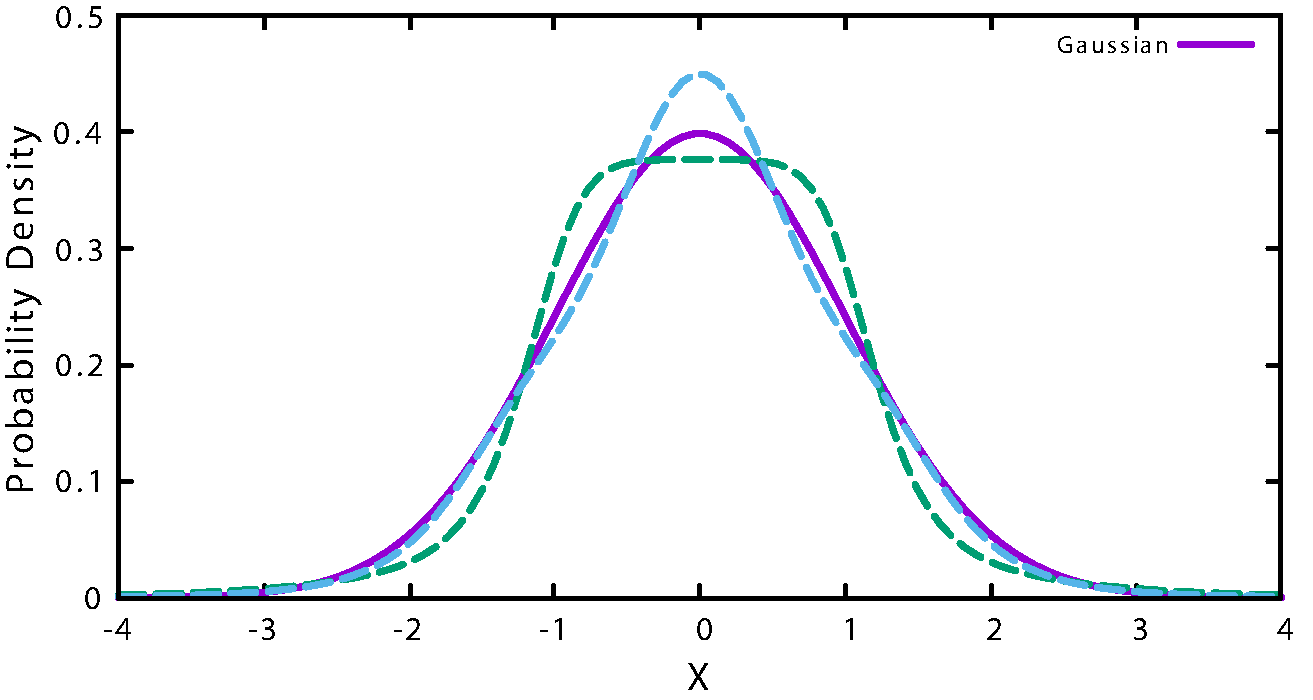
\includegraphics[width= 5in]{gauss.pdf}
  \caption{}
  \label{f:gauss}
\end{figure}

%------------------------------------------------------------------
\Section{kurtosis}
\label{s:kurtosis}

The kurtosis $\kappa_{4i}$ is defined by
\begin{equation}
  \kappa_{4i} \equiv \frac{\left< dr_i^4 \right>}{\sigma_i^4} - 3, \quad 
  i = x, y, \text{or}, z
\end{equation}
With this definition,\footnote
  {
Be aware when reading the literature that there are two definitions of kurtosis in general use. The
difference being whether three is subtracted off or not.
  }
a beam with a Gaussian distribution will have zero kurtosis. A positive kurtosis indicates more
particle in the tail than a standard Gaussian and a negative kurtosis indicates less particles.

It is important to keep in mind that the value of the kurtosis says nothing about the distribution
of particles near the center of the bunch. This is illustrated in Fig.~\ref{f:gauss}. This figure
shows three particle density curves which have been constructed to illustrate this point. The curve
drawn with a solid line is a Gaussian and the other two dashed curves are non-Gaussian. Each curve
has been constructed to have the same sigma equal to one. The Gaussian curve has a kurtosis of 0 as
expected and the other two have a kurtosis equal to 2 due to each having a tail that varies as
$1/x^6$ for $|x|$ large. Despite the two non-Gaussian curves having the same kurtosis, the shape of
the distributions in the core region are quite different with one being peaked in the center
relative to the Gaussian and the other being flattened relative to the Gaussian. To characterize the
core, there is the core emittance (\sref{s:core}).

%------------------------------------------------------------------
\Section{Data Output}
\label{s:data.out}

%------------------------------------------------------------------
\subsection{Phase Space and Action--Angle Beam Particle Data Output}
\label{s:beam.part.dat}

The phase space and action--angle data files record the particle positions in a bunch in phase space
or action--angle coordinates turn-by-turn. These files are only created if the
\vn{ltt%simulation_mode} is set to \vn{"BEAM"}. Particle data is always recorded when the beam is
at the \vn{ltt%ele_start} position independent of where the lattice begins and ends. Each line in a
file records a particle's orbital and spin position. See the Bmad manual for conversion formulas
between phase space and action-angle coordinates.

Nominally particle data is recorded every \vn{ltt%particle_output_every_n_turns} number of
turns. However, if \vn{ltt%particle_output_every_n_turns} is set to 0, particle data is recorded
only at the start and end of the tracking. If \vn{ltt%particle_output_every_n_turns} is set to -1,
particle data is only recorded at the end of tracking.

The name of the files are derived from the parameters (\sref{s:out.files}):
\begin{code}
ltt%phase_space_output_file   -- phase space file name
ltt%action_angle_output_file  -- action angle file name
\end{code}
If the file name contains a hash character ``\#'', the data file name is formed by substituting the
turn number for the hash token. If there is no hash character, the data file name is formed by
appending the turn number to the file name If there are multiple bunches, instead of using the turn
number, the substituted string will be of the form
\begin{code}
{bunch_index}-{turn_number}
\end{code}

The columns of the phase space file are:
\begin{code}
ix                      -- Particle index
turn                    -- Turn number
x, px, y, py, z, pz     -- Particle phase space 
pc, p0c                 -- Particle momentum and reference momentum.
spin_x, spin_y, spin_z  -- Spin vector
state                   -- Particle state (alive, etc.)
\end{code}

The columns of the action-angle file are:
\begin{code}
ix                      -- Particle index
turn                    -- Turn number
Ja, Angle_a             -- A-mode action and angle
Jb, Angle_b             -- B-mode action and angle
Jc, Angle_c             -- C-mode action and angle
spin_x, spin_y, spin_z  -- Spin vector
state                   -- Particle state (alive, etc.)
\end{code}

%------------------------------------------------------------------
\subsection{Beam Averages Data Output}
\label{s:beam.ave.dat}

If \vn{ltt%averages_output_file} is not blank, three data files will be produced.\footnote
  {
The reason to generate multiple data files is to avoid a file with extremely long lines.  
  }
The names of the three files will be generated by appending the suffixes ``\vn{.ave}'',
``\vn{.sigma}'', and ``\vn{.emit}'' to the name. If the \vn{ltt%averages_output_file} string
contains a hash ``\vn{\#}'' character, rather than appending the suffixes, the suffixes, minus the
beginning dot character, will be substituted for the hash mark.

Each line in a file represents beam parameters at the end of a turn and a new line is added every
\vn{ltt%averages_output_every_n_turns} number of turns. Data is always recorded when the beam is at
the \vn{ltt%ele_start} position independent of where the lattice begins and ends. If set to -1 (the
default), the output will only happen at the last turn. If set to 0, output will happen on the
beginning turn (turn 0) and the last turn.

The \vn{averages} file with the \vn{.ave} suffix will contain the following columns:
\begin{code}
Turn                          -- Turn number
N_live                        -- Number of live particles
Time                          -- Time from start
Polarization                  -- Spin polarization
<Sx>, <Sy>, <Sz>              -- Average spin components
<x>, <px>, <y>, 
      <py>, <z>, <pz>         -- Beam phase space centroid.
<pc>                          -- Average momentum (eV).
<p0c>                         -- Reference momentum
Sig_x, Sig_px, Sig_y, 
      Sig_py, Sig_z, Sig_pz   -- Phase space sigmas
\end{code}

The \vn{sigma} file with the \vn{.sigma} suffix will contain the following columns:
\begin{code}[mathescape=true]
Turn                          -- Turn number
N_live                        -- Number of live particles
Time                          -- Time from start
Sigma_Matrix                  -- Sigma matrix (21 columns)
\end{code}
The 6x6 sigma matrix $\boldsymbol{\Sigma}$ is a measure of the beam size defined by
\begin{equation}
\Sigma_{ij} = \left< dr_i \, dr_j \right>
\end{equation}
where $\bf dr$ is the deviation of the particle phase space position from the average and $<\ldots>$
denotes an average over all particles. Since the matrix is symmetric, only 21 columns are needed.

The \vn{emittance} file with the \vn{.emit} suffix will contain the following columns:
\begin{code}
Turn                          -- Turn number
N_live                        -- Number of live particles
Time                          -- Time from start
emit_a, emit_b, emit_c        -- Normal mode emittances
kurtosis_x, kurtosis_y, 
      kurtosis_z              -- Kurtosis in $x$, $y$, and $z$ directions
skew_x, skew_y, skew_z        -- Skewness in $x$, $y$, and $z$ directions
core_emit_a, core_emit_b,
      core_emit_c             -- "Core" emittance for 
core_emit_a, core_emit_b,     --            ltt%core_emit_cutoff(1)
      core_emit_c             -- "Core" emittance for
core_emit_a,                  --            ltt%core_emit_cutoff(2)
... etc...
\end{code}
Skewness $\kappa_3$ is defined by
\begin{equation}
  \kappa_{3i} \equiv \frac{\left< dr_i^3 \right>}{\sigma_i^3}, \quad 
  i = x, y, \text{or}, z
\end{equation}
And kurtosis $\kappa_4$ is covered in Section~\ref{s:kurtosis}.

%------------------------------------------------------------------
\subsection{Beam Custom Data Output}
\label{s:beam.cust.dat}

A custom output file can be created that records beam and lattice parameters every $N$\Th turn where
$N$ is set by \vn{ltt%averages_output_every_n_turns}. The columns of the file are set by the
\vn{ltt%column(:)} parameters.

Each line in a file represents beam parameters at the end of a turn and a new line is added every
\vn{ltt%averages_output_every_n_turns} number of turns. Data is always recorded when the beam is at
the \vn{ltt%ele_start} position independent of where the lattice begins and ends. If set to -1 (the
default), the output will only happen at the last turn. If set to 0, output will happen on the
beginning turn (turn 0) and the last turn.

Columns in the custom file are specified by setting \vn{ltt%column(<i>)}. The general syntax is:
\begin{code}
ltt%column(<i>) = "<expression>", "<header-name>",  "<format>"
\end{code}
where \vn{<i>} is the column index, \vn{<expression>} is an arithmetical expression that determines
the values displayed in the column, \vn{<header-name>} is a descriptive string used in constructing
the header line (first line) in the file, and \vn{<format>} is the format specifier used when
converting the value of an expression into a string. Example:
\begin{code}
ltt%column(1) = "n_turn", "N_turn", "i7"
ltt%column(2) = "rf0##1[voltage]", "Volt", "f10.0"
ltt%column(3) = "rf0##1[phi0] + z/rf0##1[rf_wavelength]", "dPhi", "es12.8"
\end{code}
Here three columns are specified. Parameters that are used in a column's \vn{<expression>} can be
element attributes or beam quantities. Using element attributes can be helpful when ramping is
used. In the above example, the second column's expression is the \vn{voltage} of the first element
named \vn{rf0} in the lattice (see the Bmad manual for lists of element parameters). Other
parameters are:
\begin{code}
n_turn      -- Turn number
time        -- Time.
x, px, y, py, z, pz
            -- Particle phase space averaged over the beam.
pc, p0c     -- Particle momentum and reference momentum
sx, sy, sz  -- Spin vector
\end{code}
Thus the third column in the above example is the averaged particle phase with respect to the zero
crossing phase of the first element named \vn{rf0} in the lattice. [Note that $z$ is always evaluated
at the start of the turn and not at the position of the RF cavity.]

%------------------------------------------------------------------
\Section{Spin Tracking Damping Time and Polarization Analysis}
\label{s:spin.track}

Long term tracking including spin is often used to calculate damping times and equilibrium
polarizations. One common strategy is to first track a beam for a few damping times until it has
reached equilibrium in the orbital phase space. The beam distribution is now saved and a new run
is started with this saved orbital distribution and with all the spins aligned so that the
beam is 100\% polarized. A plot of polarization vs time now gives the damping time. See the section
in the Bmad manual on ``Polarization Limits and Polarization/Depolarization Rates''.

%------------------------------------------------------------------
\Section{Some Checks to be Done if Particles Cannot be Stability Tracked}

There can be any number of reasons why particles cannot be stably tracked over many turns. The
following are some checks that can be done.
\begin{itemize}
\item
Check for a resonance condition $l\,Q_x + m\,Q_y + n\,Q_z = p$. The \vn{show universe} command in
Tao will show the tunes. The \vn{tune_plane_res_plot} program can be used to plot resonance lines in
the $(Q_x, Q_y)$ tune plane. Also the \vn{tune_scan} program can be used to see where
the beam blows up in the $(Q_x, Q_y)$ tune plane.
%
\item
Check that radiation damping and excitation are both on or both off.
%
\item
Check that the RF voltage is sufficient considering the average radiation loss plus the energy sigma
of the beam.
%
\item
If using PTC or MAP tracking, check that enough slices are being used to accurately model the lattice
%
\item
Check that lattice is stable. To do this, check that the damping partition numbers are all
positive. The damping partition numbers can be seen using the Tao program's \vn{show universe}
command. Note: Make sure that in Tao that the radiation damping and RF on/off match what is being used in
the long_term_tracking program.
%
\item
Using SINGLE mode tracking, output a turn-by-turn orbit by setting:
\begin{code}
ltt%phase_space_output_file = "some-nonblank-name" 
ltt%particle_output_every_n_turns = 1
\end{code}
Use your favorite plotting program to plot the phase space trajectory. This will give a lot of information. For
example, look to see in which plane an instability starts.
\end{itemize}

%------------------------------------------------------------------
\begin{thebibliography}{9}

\bibitem{b:bmad}
D. Sagan,
``Bmad: A Relativistic Charged Particle Simulation Library''
Nuc.\ Instrum.\ \& Methods Phys.\ Res.\ A, {\bf 558}, pp 356-59 (2006).

\bibitem{b:ptc}
É. Forest, Y. Nogiwa, and F. Schmidt. The FPP and PTC libraries. In Int.\ Conf.\ Accel.\
Phys pp 17–21, (2006).

\bibitem{b:wolski}
A. Wolski, "Alternate approach to general coupled linear optics",
Phys.\ Rev.\ Special Topics, Accel \& Beams, {\bf 9}, 024001 (2006).

\bibitem{b:gulliford}
Colwyn Gulliford, Adam Bartnik, Ivan Bazarov, Bruce Dunham, and Luca Cultrera,
``Demonstration of Cathode Emittance Dominated High Bunch Charge Beams in a DC gun-based Photoinjector'',
Appl. Phys. Lett. {\bf 106}, 094101 (2015). https://doi.org/10.1063/1.4913678

\end{thebibliography}

\end{document}

